\section{Migragrea clienților}

\begin{frame}{Migrarea clienților}
  \begin{itemize}
    \item Mecanismul de handoff e folosit și pentru balansarea încărcării AP-urilor
    \item Se folosește metrica capacității disponibile
  \end{itemize}
\end{frame}

\begin{frame}{Mecanismul de handoff}
  \begin{columns}
  \begin{column}{0.5\linewidth}
    \begin{enumerate}
      \item DC adaugă MAC-ul clientului pe DAP2
      \item DAP2 trimite un mesaj proxy ARP cu IP-ul său
      \item DC îi cere lui DAP1 să trimită un frame de dezasocierelui C
      \item DAP1 scoate clientul din ACL și trimite frame-ul
      \item Clientul începe să caute alt AP
      \item DAP2 răspunde clientului
    \end{enumerate}
  \end{column}
  \begin{column}{0.5\linewidth}
    \begin{figure}
      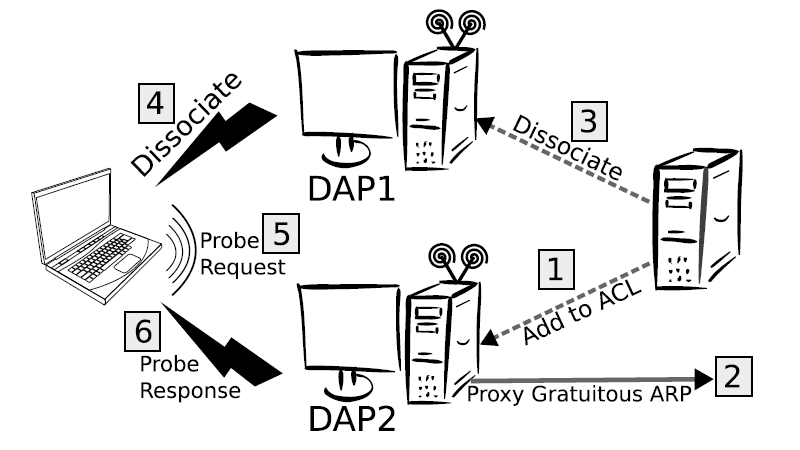
\includegraphics[scale=0.20]{img/fig3.png}
    \end{figure}
  \end{column}
  \end{columns}
\end{frame}

\begin{frame}
\begin{itemize}
  \item Balansarea încărcării AP-urilor
  \begin{itemize}
    \item Este posibil ca starea sistemului să se schimbe sau estimarea inițială să nu fie exactă
    \item Dacă încărcarea pe un AP devine prea mare, se mută clienții, unul câte unul, pe alte AP-uri, astfel încât să se mențină un throughput ridicat
    \item Trebuie minimizat numărul de handoff-uri deoarece sunt evenimente disruptive pentru client
  \end{itemize}
  \item Mobilitate
  \begin{itemize}
    \item DC-ul poate determina locația clientului
    \item Dacă clientul se mută mai mult de 10 metri DC-ul poate să reasocieze clientul la un alt AP, dacă există unul mai bun
  \end{itemize}
\end{itemize}
\end{frame}

